% Boilerplate and packages
\documentclass[a4paper,12pt]{article}
\usepackage{latexsym, amsmath, amssymb, amsfonts, amsthm}
\usepackage{graphicx, float}
\usepackage[utf8]{inputenc}
\usepackage{polski}
\usepackage[skip=10pt plus1pt, indent=0pt]{parskip}
%\usepackage{XCharter} % Fajna czcionka
%\usepackage{geometry} % Zmień układ dokumentu
%\geometry{
% a4paper,
% left=30mm,
% right=30mm,
% top=30mm,
% bottom=30mm
%}

\frenchspacing
\newtheorem{definition}{Definicja}
\newtheorem{theorem}{Twierdzenie}
\theoremstyle{remark}
\newtheorem{example}[definition]{Przykład}

% Title details
\title{Wstęp do matematyki}
\author{}
\date{}

% Actual document
\begin{document}
\maketitle

\section{Indukcja matematyczna}

\textit{Zasada indukcji matematycznej} jest jednym z ważniejszych sposobów dowodzenia (lub definiowania) własności liczb naturalnych, znajdującym liczne zastosowania w każdym dziale matematyki. Sposoby dowodzenia własności matematycznych, w których korzysta się z zasady indukcji matematycznej, nazywa się sposobami indukcyjnymi, a same dowody – \textit{dowodami indukcyjnymi}. W każdym takim pojedynczym dowodzie w skończonym czasie jednocześnie wykazujemy prawdziwość nieskończenie wielu zdań.

Przedstawimy teraz indukcyjny dowód wzóru na sumę sześcianów kolejnych liczb naturalnych.

\begin{example}
    Udowodnić, że dla każdej dodatniej liczby naturalnej $n$ mamy:
    \begin{equation}
        1^3 + 2^3 + \cdots n^3 = \frac{n^2(n+1)^2}{4}.
    \end{equation}
\end{example}

Równość (1) jest prawdziwa dla $n=1$, bo $1^3=1=1^2(1+1)^2/4$. Założmy teraz, że $n$ jest pewną dodatnią liczbą naturalną i przypuśćmy, że dla tej liczby mamy
\begin{equation}
    1^3 + 2^3 + \cdots n^3 = \frac{n^2(n+1)^2}{4}.
\end{equation}

Udowodnimy, że wtedy także mamy
\begin{equation*}
    1^3 + 2^3 + \cdots (n+1)^3 = \frac{(n+1)^2(n+2)^2}{4}.
\end{equation*}

\newpage

Istotnie mamy
\begin{eqnarray*}
     1^3 + 2^3 + \cdots + (n+1)^3 & = & (1^3 + 2^3 + \cdots + n^3) + (n+1)^3 \\
     & = & \dfrac{n^2(n+1)^2}{4} + (n+1)^3 \text{ (z założenia 2)} \\
     & = & \dfrac{(n+1)^2(n+2)^2}{4}
\end{eqnarray*}

Z powyższego i z zasady indukcji matematycznej wynika prawdziwość równości (1) dla każdej dodatniej liczby naturalnej $n$.

Powyższy rozdział powstał na podstawie \cite{WDM}.

\section{Podzbiory}

\begin{definition}
    \label{podzbior}
    Mówimy, że zbiór $A$ jest podzbiorem zbioru $B$, piszemy $A \subseteq B$, wtedy i tylko wtedy, gdy każdy element zbioru $A$ jest elementem zbioru $B$, czyli mamy
    \begin{equation}
        A \subseteq B \Leftrightarrow \forall_x \ [x \in A \Rightarrow x \in B].
    \end{equation}
\end{definition}

Symbol $\subseteq$ nazywamy znakiem inkluzji lub znakiem zawierania. Fakt, że zbiór $A$ nie jest podzbiorem zbioru $B$, wyrażamy zapisem $A \nsubseteq B$. Zatem wobec (3), prawa eliminacji implikacji i prawa de Morgana dla alternatywy, mamy
\begin{equation}
    A \nsubseteq B \Leftrightarrow \exists_x \ [x \in A \land x \notin B].
\end{equation}

\begin{example}
    $\{a,b\} \subseteq \{a,b,c\}$ i $\{1,2,3\} \nsubseteq \{1,3,5\}$.
\end{example}

Udowodnimy teraz, że inkluzja zbiorów jest przechodnia (i dziedziczna).

\begin{theorem}
    Jeśli $A, B$ i $C$ są zbiorami takimi, że $A \subseteq B$ i $B \subseteq C$, to $A \subseteq C$.
\end{theorem}

\begin{proof}
    Załóżmy, że $A \subseteq B$ i $B \subseteq C$. Weźmy dowolny element $x \in A$.
    Ponieważ $x \in A$ i $A \subseteq B$, więc wobec definicji \ref{podzbior} wnioskujemy, że $x \in B$.
    Teraz $x \in B$ i $B \subseteq C$, więc znowu korzystamy z definicji \ref{podzbior} i tym razem
    wnioskujemy, że $x \in C$. To kończy dowód inkluzji $A \subseteq C$.
\end{proof}

\newpage

\subsection{Diagramy Venna}

Zbiory warto ilustrować za pomocą rysunków nazywanych diagramami Venna. W tych ilustracjach zbiory reprezentowane są najczęściej przez koła, elipsy lub prostokąty. Ilustracje te są źródłem pierwszych obserwacji, intuicji i pierwszych własności działań na zbiorach. Umieszczając ilustrację zbioru $A$ wewnątrz ilustracji zbioru $B$ (tak jak to zrobiliśmy na rys. 1), graficzne wyrażamy fakt, że $A$ jest podzbiorem zbioru $B$.

\begin{figure}[h]
    \centering
    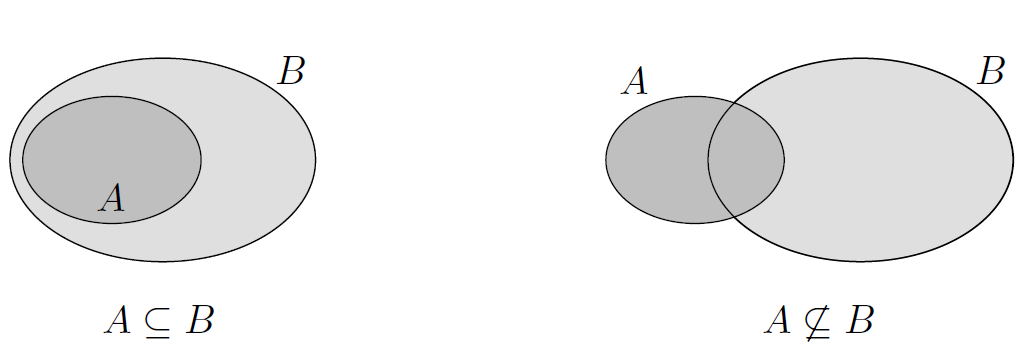
\includegraphics[width=\textwidth]{diagramy.png}
    \caption{Diagram Venna}
\end{figure}

\section{Podsumowanie}

Na zajęciach z {\LaTeX} korzystaliśmy z \cite{NZKWDSL}. Można tam znaleźć na przykład następujący wzór:

\begin{equation*}
    \left(
        \begin{array}{c|c}
            1 & 2 \\
            \hline
            3 & 4
        \end{array}
    \right)
\end{equation*}

\newpage

\begin{thebibliography}{00}
    \bibitem{WDM}
        J. Topp: \textit{Wstęp do matematyki}, wydawnictwo PG, Gdańsk 2009.
    \bibitem{NZKWDSL}
        Nie za krótkie wprowadzenie do systemu {\LaTeX}.
\end{thebibliography}

\end{document}